\subsection{Results}

We provide some results from the experiment. Given the preliminary nature
of the experiment, these results serve mostly as a benchmark to help
understand possible usefulness and guide future efforts. To measure our results,
throughout our experiment, for each click generated by the user, we recorded
its position, timestamp, whether it was in a target or not, what pointing
mode they were in, sensitivity, and smoothing factor. From this information, we
are able to calculate the accuracy of a user through a given trial, as well
as time taken. We additionally expected that participants would toggle between
pointing modes and adjust sensitivity on the fly, which would provide us
data points for further tuning our initial estimates. For the Fitts' task,
we compare the time taken and accuracy against an ``index of
difficulty'', which is calculated via Fitts' Law:

\begin{equation}
    ID = log_{2}(\frac{2 * D}{W})
\end{equation}

where $D$ is the distance between the center of the bars and $W$ is the rectangle
width. The expectation here is that as $ID$ increases, the accuracy would fall,
and time taken would increase. The $ID$ for our experimental set-up ranged from
4.32 and 6.87. Our results of mean accuracy is shown in
Figure~\ref{fig:user_study_fitts_accuracy}, mean time taken is shown in
Figure~\ref{fig:user_study_fitts_time_taken}. For this task, we also provide
a measure of the mean ``reaction time'' (RT) which was the amount of time
taken between successive correct clicks on the bars, which is shown in
Figure~\ref{fig:user_study_fitts_rt}

For the second task, our accuracy  to the task was 78\% and time taken was 
48.18s. After both tests, the results from our NASA TLX  are shown in
Table~\ref{table:muifold_tlx}. Throughout the entire experiment, users
ended up choosing not to toggle between pointing modes (we did not insist
to users that they should) nor did they really adjust the sensitivity or
smoothing beyond a point or two away from the provided default. In our
pre-survey, all users stated that they had familiarity with using most of the
range of devices except that no user had used cellphones as pointers before.
Only one user indicated that they had prior experience with ``smart rooms''
before.


\begin{figure}
\centering
  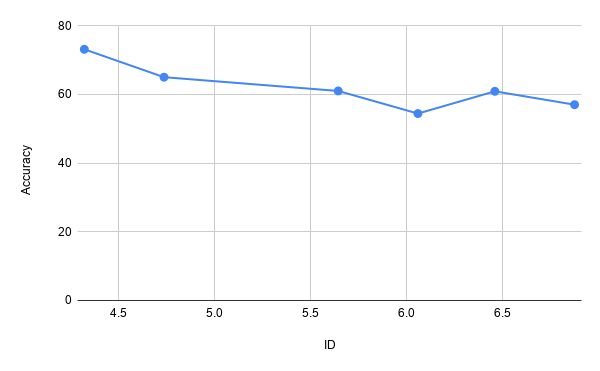
\includegraphics[width=0.6\columnwidth]{chapters/04_muifold/figures/user_study_chart_id_accuracy.png}
  \caption{The participants' mean task accuracy for Fitts' task as a function of index of difficulty.}
  \label{fig:user_study_fitts_accuracy}
\end{figure}

\begin{figure}
\centering
  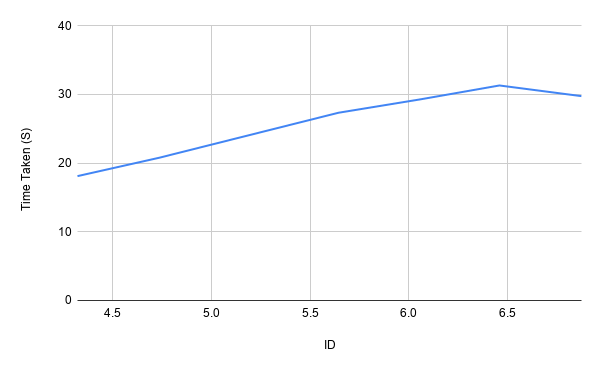
\includegraphics[width=0.6\columnwidth]{chapters/04_muifold/figures/user_study_fitts_time_taken.png}
  \caption{The participants' mean time taken for Fitts' task as a function of index of difficulty.}
  \label{fig:user_study_fitts_time_taken}
\end{figure}

\begin{figure}
\centering
  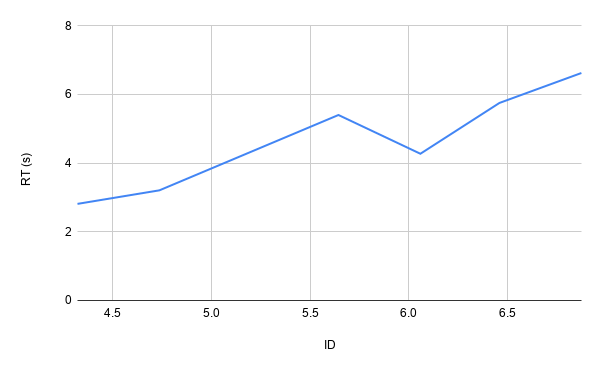
\includegraphics[width=0.6\columnwidth]{chapters/04_muifold/figures/user_study_fitts_rt.png}
  \caption{The participants' reaction time for Fitts' task as a function of index of difficulty.}
  \label{fig:user_study_fitts_rt}
\end{figure}

\begin{table}[hbtp]
    \centering
    \caption{Averaged results from NASA TLX, scores ranged from -10 to 10, lower is better.}
    \begin{tabular}{ |c|c| }
         \hline
         Mental Demand & -6 \\
         \hline
         Physical Demand & -3.5 \\
         \hline
         Temporal Demand & -6.5 \\
         \hline
         Performance & -4.5 \\
         \hline
         Effort & 2.75 \\
         \hline
         Frustration & 3 \\
        \hline
    \end{tabular}
    
    \label{table:muifold_tlx}
\end{table}